\documentclass[a4paper,11pt,UTF8]{article}
\usepackage{ctex}
\usepackage{amsmath,amsthm,amssymb,amsfonts}
\usepackage{amsmath}
\usepackage[a4paper]{geometry}
\usepackage{graphicx}
\usepackage{microtype}
\usepackage{siunitx}
\usepackage{booktabs}
\usepackage[colorlinks=false, pdfborder={0 0 0}]{hyperref}
\usepackage{cleveref}
\usepackage{esint} 
\usepackage{graphicx}
\usepackage{ragged2e}
\usepackage{pifont}
\usepackage{extarrows}
\usepackage{mathptmx}
\usepackage{float}
\usepackage{caption}
\usepackage{subfigure}

\captionsetup[figure]{name={Figure}}

\title{Microelectronics Circuit Analysis and Design Homework(15th)}
\author{Yuejin Xie \quad U202210333}
\date{Nov 15th, 2023}
\begin{document}
\maketitle
15.15 Consider the bandpass filter in Figure P15.15.(a) Show that the voltage transfer function is
$$
A_v(s)=\frac{v_O}{v_I}=\frac{-1/R_4}{(1/R_1)+sC+1/(sCR_2R_3)}
$$
(b) For $C= 0.1$ μF, $R_1=85$ k$\Omega,\quad R_2=R_3=300\Omega,\quad R_4=3$ k$\Omega$, and
$R_5=30$ k$\Omega$, determine: (i) $|A_v( $max$) |; $(ii) the frequency $f_o$ at which $|A_v( $max$) |$ occurs; and (iii) the two 3 dB frequencies.
\begin{figure}[H]
	\centering
	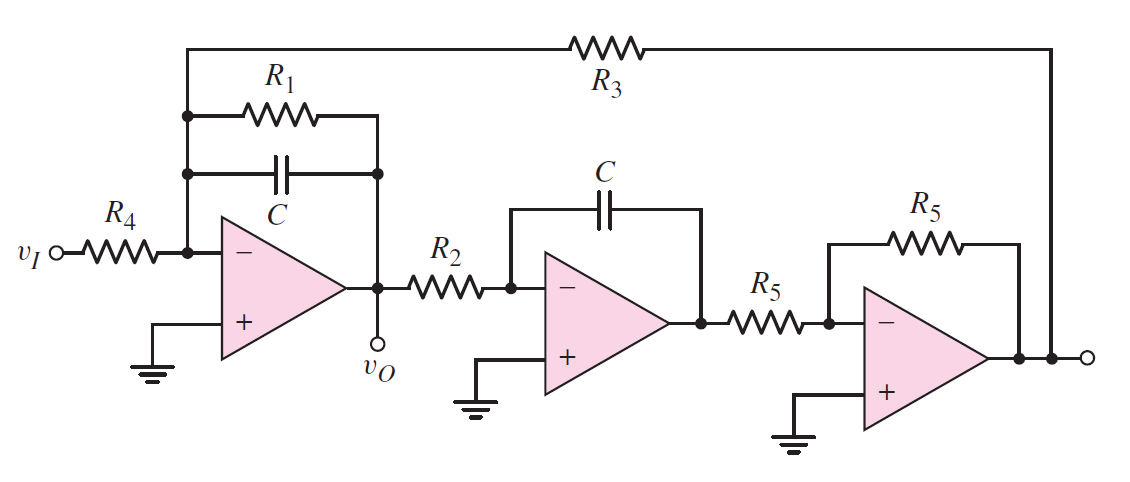
\includegraphics[width=0.6\textwidth]{15.15}
	\caption{Problem 15.15}
\end{figure}

15.17 For each of the circuits in Figures P15.17, derive the expressions for the voltage transfer function $T(s)=V_o(s)/V_i(s)$ and the cutoff frequency $f_{3\text{dB}}.$
\begin{figure}[H]
	\subfigure[]{
		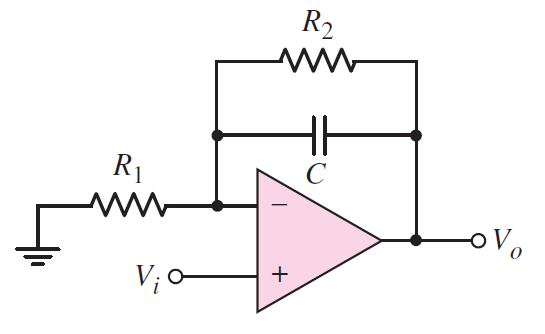
\includegraphics[width=0.4\textwidth]{15.17_a}
	}
	\subfigure[]{
		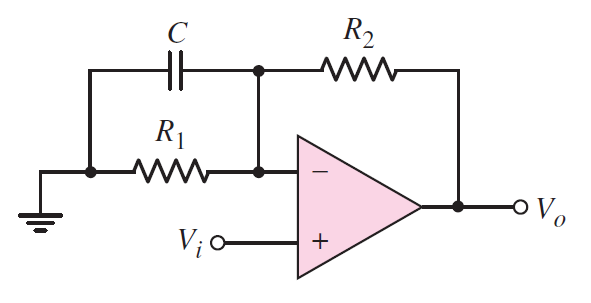
\includegraphics[width=0.4\textwidth]{15.17_b}
	}
	\centering

	\caption{Problem 15.17}
\end{figure}
15.46 Consider the Schmitt trigger in Figure P15.46. Assume the saturated output voltages are $\pm V_P.$ (a) Derive the expression for the crossover voltages $V_{TH}$ and $V_{TL}$. (b) Let $R_A=10$ k$\Omega$, $R_B=20$ k$\Omega,\:R_1=5$ k$\Omega,\:R_2=20$ k$\Omega$, $V_P=10$ V, and $V_{\mathrm{REF}}=2$ V. (a) Find $V_{TH}$ and $V_{TL}.( $b$) $ Sketch the voltage transfer characteristics.
\begin{figure}[H]
	\centering
	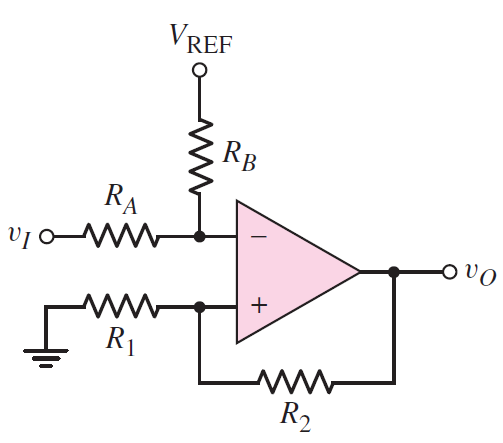
\includegraphics[width=0.4\textwidth]{15.46}
	\caption{Problem 15.46}
\end{figure}
15.47 The saturated output voltages are $\pm V_P$ for the Schmitt trigger in Figure P15.47. (a) Derive the expressions for the crossover voltages $V_{TH}$ and  $V_{TL}$ (b) If $V_P= 12$V, V REF$= - 10$V, and $R_3= 10$k$\Omega$, find $R_1$ and $R_2$ such that the switching point is $V_S=-5$ V and the hysteresis width is O.2 V. (c) Sketch the voltage transfer characteristics.
\begin{figure}[H]
	\centering
	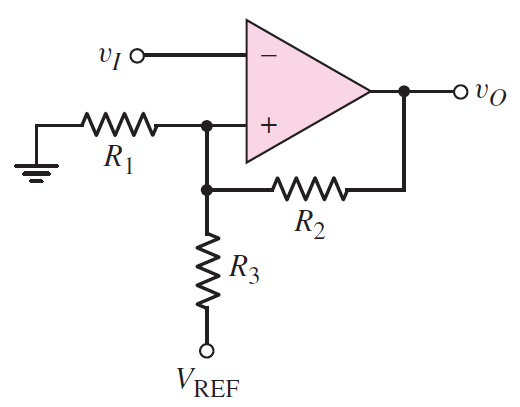
\includegraphics[width=0.4\textwidth]{15.47}
	\caption{Problem 15.47}
\end{figure}
15.48 (a) Plot the voltage transfer characteristics of the comparator circuit in Figure P15.48 assuming the open-loop gain is infinite. Let the reverse Zener voltage be $V_{Z}=5.6$ V and the forward diode voltage be $V_{\gamma}=0.6$ V. (b) Repeat part (a) for an open-loop gain of $10^3.(c)$ Repeat part (a) for 2.5 V
applied to the inverting terminal l of the comparator.
\begin{figure}[H]
	\centering
	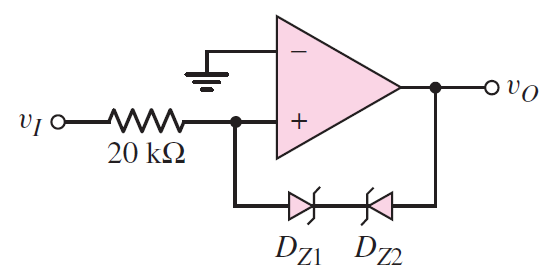
\includegraphics[width=0.4\textwidth]{15.48}
	\caption{Problem 15.48}
\end{figure}
	
\end{document}